\chapter{Marco Teórico}
\section{Fatiga}

El fenómeno en el cual una estructura se daña e incluso falla por cargas fluctuantes, es llamado fatiga. El estudio de este problema comenzó tempranamente en europa durante la mitad del siglo XIX, en pleno auge de la industralización europea, producto de la falla repentina de algunos componentes en máquinas y los ejes de los trenes de la época. Estos experimentaban un gradual debilitamiento de la resistencia, fallando aún cuando su esfuerzo último no fuese alcanzado. 

Así, en 1837 fueron publicados los resultados del primer ensayo de fatiga, realizado a una cadena transportadora utilizada en minas de hierro en Alemania. Wilhelm Albert, quien realizó esta investigación, se vió motivado a realizar los estudios por los altos costos que significaba la falla de este componente producto de las cargas cílicas a las que estaba sometida. Los pocos conocimientos existentes del fenómeno en esa época, llevo a que la solución al problema fuese la invención del cable de acero.

Por otro lado, las primeras investigaciones enfocadas a comprender el fenómeno comenzaron en 1858 con August Wölher. Su acucioso estudio lo llevó a conclusiones que siguen teniendo importancia y validez hasta el día de hoy. Diseñó, durante la década de 1860, una máquina de ensayos de flexión y flexión rotativa. En 1870 presentó un informe en el cual parte de sus conclusiones cualitativas son llamadas ``Ley de Wöhler'', al establecer el esfuerzo alternante como el parámetro más importante para la vida de un componente, señalanado que ``the stress amplitudes are decisives for the destruction of the cohesion of the material. The maximum stress is of influence only in so far as the higher it is, the lower are the stress amplitudes which lead to failure''\textcolor{red}{citar schutz history of fatigue}, aunque destacando también que el esfuerzo medio tiene una influencia perjudicial en el material. 

Es decir, desde 1853 hasta hoy, han transcurrido más de 160 años de investigación sobre la fatiga, logrando comprender distintas aristas del fenómeno, pero con muchas preguntas aún sin resolver. Por eso, la fatiga sigue siendo un problema necesario de abordar y seguir comprendiendo, por sus grandes implicaciones de costo que tiene en la industria y en distintos elementos que utilizamos en la vida diaria. Por otro lado, si bien muchas preguntas no han sido resueltas científicamente, diversas empresas han logrado evitar las fallas por fatiga y optimizar los diseños de manera operativa, sin comprender cabalmente el trasfondo de estos.  



\subsection{Definiciones}
La fatiga se puede definir, desde la perspectiva del material, como el proceso en el cual el daño se acumula producto de la aplicación de cargas repetitivas que se encuentran bajo el punto de fluencia. En metales, este proceso se divide en tres fases o etapas las cuales, dependiendo del autor, pueden ser llamadas: fase de iniciación de la grieta, fase de crecimiento de la grieta y fractura.

La primera fase es el inicio de una o más microgrietas, la cual ocurre tempranamente en la vida a fatiga de un material y que, incluso, pueden ocurrir inmediatamente si el esfuerzo cíclico se encuentra sobre el límite de fatiga. Lo característico de esta etapa es que las grietas no pueden verse a simple vista, fase que representa una parte considerable de la vida a fatiga total. Estas crecerán lentamente y de manera errática, debido al efecto de las microestructuras como los bordes de grano. Durante este período, las concentraciones de esfuerzo juegan un importante papel, al ser los lugares donde comenzará la nucleación de las grieta, sumado a las pocas restricciones de deslizamiento de la superficie del material, hace que esta sea relevante en el inicio de este proceso.

En la segunda etapa, las microgrietas pasan a ser macrogrietas, es decir, son visibles al ojo humano. Estas grietas comienzan a tomar una dirección de crecimiento que es perpendicular a los esfuerzos principales producidos por la carga alternante. La resistencia al crecimiento de las grietas, cuando esta penetra el material, dependerá de las propiedades de grano. Así, se puede definir cualitativamente una separación entre ambas etapas, donde el periodo de iniciación o nucleación de las grietas termina cuando su crecimiento no es dependiente de las condiciones superficiales del material. Producto de la micro-deformación plástica cíclica se forman bandas de crecimiento conocidos como \textit{marcas de playa} o \textit{``striations patterns''}, abriendo, cerrandose y frotandose entre sí, como se puede ver en la imagen \textcolor{red}{Añadir figura 2.24 de Fatigueofstructuresandmaterial 2009}, dejando en evidencia el frente de grieta, las variaciones en la carga, su velocidad de crecimiento y la naturaleza corrosiva del entorno.

Finalmente, la última etapa es la falla del material, que ocurre en el último ciclo de la carga, al no poder soportarla con el material restante. Esta fractura es rápida y es producto de una macro-deformación plástica, pudiendo ser frágil, dúctil o una combinación de ambas.

Con esto en cuenta, es posible definir ciertos conceptos en base a las distintas etapas que experimenta un material. La vida a fatiga de un material (\textit{fatigue life}, $N_f$) es el número de ciclos aplicados a una probeta para lograr el criterio de falla \textcolor{red}{referencia a ISO 23718}. El límite de resistencia a la fatiga (\textit{endurance limit}) es frecuentemente explicado como la amplitud de esfuerzo para el cual la vida a fatiga tiende a infinito o a la asíntota de la curva S-N. Sin embargo, al comprender la fatiga como un proceso, es posible dar una definición más acertada para el límite a la fatiga, pasando a ser el umbral para el crecimiento de las microgrietas. Es decir, bajo este límite existe nucleación e iniciación de grites, sin embargo, su crecimiento está limitado a los bordes de grano del material.

Por otra parte, para el estudio de este fenómeno existen tres modelos de falla por fatiga: de \textit{esfuerzo-vida} ($S$-$N$), de \textit{deformación-vida }($\varepsilon$-N) y de la \textit{mecánica de fractura lineal elástica} (LEFM). Cada uno de ellos tiene ventajas y desventajas, sin embargo, la máquina que es objeto de evaluación en este trabajo utiliza el método \textit{esfuerzo-vida}. El criterio de elección entre los distintos modelos se divide principalmente por la cantidad de ciclos que se hará la medición, los que se clasifican en régimen de fatiga de ciclo bajo (\textit{low-cycle fatigue}, LCF) o un régimen de fatiga de ciclo alto (\textit{high-cycle fatigue}, HCF). La división entre ambos régimen dependerá de distintos autores, no obstante, por lo general se establece la separación en $10^3 \leq LCF$ y $10^3 > HCF$ \textcolor{red}{referencia al shigley - pag. 265}, debido a que la zona LCF está asociada a la existencia de macro-deformaciones plásticas en cada ciclo. De esta manera, el método de esfuerzo-vida se utiliza para ensayos de alto ciclaje debido a su poca precisión en casos LCF. A su vez, los métodos de deformación-vida y LEFM se aplican para casos LCF.

En el método de esfuerzo-vida las muestras o probetas son sometidas a fuerzas de magnitudes especificadas, al mismo tiempo que se cuentan la cantidad de ciclos. Es por esto que es un modelo con base en el esfuerzo, con el cual se busca determinar una resistencia de fatiga o un límite de resistencia a la fatiga. 

Estas fuerzas especificadas pueden ser constantes o variables en el tiempo y magnitud, sin embargo, se abordará principalmente los casos donde los esfuerzos fluctúan de manera constante en el tiempo y de una amplitud fija debido a las características de la máquina analizada en este trabajo. Esto permite trazar la curva de fatiga (S-N) del componente o material para distintas cargas con su respectivo número de ciclos que falla.

Por esto, se hace necesario describir y definir elementos que surgen producto de una carga cíclica. Esta se caracteriza por el esfuerzo alternante (\textit{alternate stress} o \textit{amplitude stress}, $S_a$) y el esfuerzo medio (\textit{mean stress}, $S_m$) que se muestran en la ecuación \ref{eq:s_a} y \ref{eq:s_m}, respectivamente. A su vez, estas se definen por el esfuerzo máximo $S_{max}$ y $S_{min}$, siendo el esfuerzo máximo y mínimo alcanzado por la carga cíclica. Finalmente, el rango del esfuerzo, $\Delta S$ (eq. \ref{eq:ds}), y la razón de esfuerzos, $R$ (eq. \ref{eq:r_s}), también son opciones  para caracterizar la fatiga.

\begin{align}
	S_a &= \frac{S_{max} - S_{min}}{2} \label{eq:s_a} \\
	S_m &= \frac{S_{max} + S_{min}}{2} \label{eq:s_m} \\
	\Delta S &= S_{max} - S_{min} = 2S_a  \label{eq:ds} \\
	R &= \frac{S_{min}}{S_{max}} \label{eq:r_s} 
\end{align}

Estos términos se pueden ver claramente en la figura \textcolor{red}{Insertar imagen que muestra Sa Sm etc}. Existen dos casos específicos, el primero en donde $S_m = 0$, y así $R=-1$, se llama esfuerzo de ciclo invertido. El segundo, cuando $S_{min}=0$, y $R=0$, se llama esfuerzo repetido.

\subsection{Curva S-N o de Wöhler}
Como se señaló en el punto anterior, la curva S-N es el resultado de la aplicación del método esfuerzo-vida. Es quizás uno de las herramientas más importantes en el desarrollo empírico para lograr cuantificar el proceso de fatiga y poder diseñar contra este. El diagrama S-N se obtiene como resultado de un número de ensayos de fatiga a distintos niveles de esfuerzo, donde $S$ puede ser la amplitud ($S_a$), el rango de esfuerzo ($\Delta S$) o el esfuerzo máximo ($S_{max}$) que es aplicado a la probeta, siendo la amplitud lo más común. La variable $N$ hace referencia a la vida a fatiga del material, es decir, la cantidad de ciclos hasta que la probeta falle. Debido a que se desea analizar fallas en LCF y HCF, la cantidad de ciclos necesarios para fallar la probeta pueden llegar a ser demasiado altos, por esto, $N$ se grafica en escala logarítmica.

La cantidad de ensayos requeridos para construir la curva S-N dependerá de distintos factores como, por ejemplo, la confiabilidad esperada, el uso final de la información o de los recursos disponibles. La norma E739-10 -- "Statistical Analysis of Linear or Linearized Stress-Life ($S$-$N$) and Strain-Life ($\varepsilon$-$N$) Fatigue Data", establece una guía dependiendo del tipo de prueba a realizar como se muestra en al tabla \ref{tab:type_test}. Además, se recomienda realizar la medición con, al menos, tres puntos de esfuerzos distintos. Con esto, es posible obtener el diagrama $S-N$ como el que se puede apreciar en la figura \textcolor{red}{Añadir figura 6-10, Shigley, pag 266}, donde se puede apreciar la diferencia entre la zona LCF, HCF y de vida infinita, para el caso de los aceros.


\begin{table}[]
\begin{center}
\caption{Número mínimo de pruebas según tipo de prueba}
\label{tab:type_test}
\begin{tabular}{@{}lc@{}}
\toprule
\multicolumn{1}{c}{Tipo de prueba}                                                                                        & Cantidad mínima de probetas \\ \midrule
\begin{tabular}[c]{@{}l@{}}Preliminar y exploratorio (investigación exploratoria \\ y ensayos de desarrollo)\end{tabular} & 6 a 12                      \\
\begin{tabular}[c]{@{}l@{}}Pruebas de desarrollo e investigación de componentes \\ y probetas\end{tabular}                & 6 a 12                      \\
Datos de diseños permisibles                                                                                              & 12 a 24                     \\
Datos de confiabilidad                                                                                                    & 12 a 24                     \\ \bottomrule   
\end{tabular}
\end{center}
\end{table}

La curva $S$-$N$ varía ámpliamente sus resultados para distintos tipos de materiales y, a su vez, estos se ven afectados por una variedad de factores. Estos pueden ser por modificaciones en las condiciones de ensayo, de la geometría de la probeta, de la naturaleza del material o de la forma de fabricación de la probeta. Todos estos factores crean ciertas tendencias en la obtención de datos que los distinguen unos de otros. 

En concreto, las condiciones medioambientales hostiles, ya sean químicas o térmicas, pueden acelerar el proceso de iniciación y crecimiento de grietas. Una probeta sometida a creep, fatiga y altas temperaturas puede disminuir drásticamente sus vida útil y, por tanto, la vida a fatiga del material. También es posible realizar ensayos en una solución de sal para homologar las condiciones marinas, afectando también su vida a fatiga. Otro factor que afecta los resultados de los ensayos es la frecuencia de los ciclos de carga ejercidos, al aumentar la temperatura de la probeta durante su ensayo. \textcolor{red}{Agregar imagen, pag. 387 y 388 - Dowling}

El esfuerzo residual también tiene incidencia en la curva de Wöhler, la cual puede incluso ser beneficiosa al utilizar técnicas como el granallado (\textit{shot peening}). El mecánizado de las piezas, como en el caso de la probeta utilizada por la máquina de fatiga, verá afectado los resultados de la curva $S$-$N$ dependiendo de las características con las que sea manufacturado. Como se indicó anteriormente, la primera etapa de la fatiga, la inicación de las grietas, es un fenómeno que depende de la superficie del material y como consecuencia, un mecánizado grueso o fino tendrá un impacto en esa etapa de la fatiga y no en la posterior, como se puede apreciar en la imagen \textcolor{red}{Imagen página 54 - Book of fatigue}. Así, aquellas probetas que tengan una mejor calidad superficial producto del afinado, tendrán una mejor resistencia a la fatiga respecto a otras.

Es posible encontrar otros factores que inciden en los resultados de la curva, como pueden ser la geometría de la probeta o componente, sus dimensiones, el esfuerzo último ($\sigma_{uts}$), su microestructura, tratamientos químicos y el esfuerzo medio ($S_m$). Este último será analizado en la sección siguiente, debido a la importancia que posee al estar presente en la máquina a analizar. 

%En último término, existen distintas formas de obtener la información necesario con el método esfuerzo-vida, ya sea por pruebas de fatiga axial, torsión, torsión-flexión, flexión o flexión en voladizo. Este último, es el utilizado por la máquina existente en el laboratorio de tecnología mećanica. 
%
%
%%al ser este método el más utilizado existe una gran cantidad de datos para distintos materiales, configuraciones o elementos mecánicos. Con esto resulta más fácil poder comparar resultados o encontrar información al momento de diseñar componentes que sufrirán fatiga. Por otro lado, 

\subsection{Esfuerzo medio, $S_m$}
Como se escribió anteriormente, el esfuerzo medio tiene influencia en los resultados de la curva $S$-$N$, dependiendo del tipo de ensayo realizado, con tal de lograr comparar los datos obtenidos entre distintas pruebas realizadas, como se muestra en la figura \textcolor{red}{añadir imagen 925  Dowling}. Para esto, se han desarrollado ecuaciones que buscan estimar el efecto una carga media dada cuando no existe información disponible.

Existen distintas maneras de representar la información de un ensayo donde $S_m \neq 0$. Una forma es recolectar la información de distintos ensayos con distintos valores de carga media y graficarlos como se muestra en la figura \textcolor{red}{añadir imagen anterior como rf}. Una segunda opción es realizar un diagrama de vida constante (\textit{constant fatigue life diagram}, $CFL$), mostrada en la figura \ref{fig:diag_cfl}, el cual muestra claramente que un incremento del esfuerzo medio tiene como resultado una disminución del esfuerzo alternante, para la misma vida de la probeta, $N_f$. Finalmente, es posible graficar un ensayo para distintos valores de $R$, como se muestra en la figura \textcolor{red}{imagen 935 Dowling}.

\begin{figure}[h]
\centering
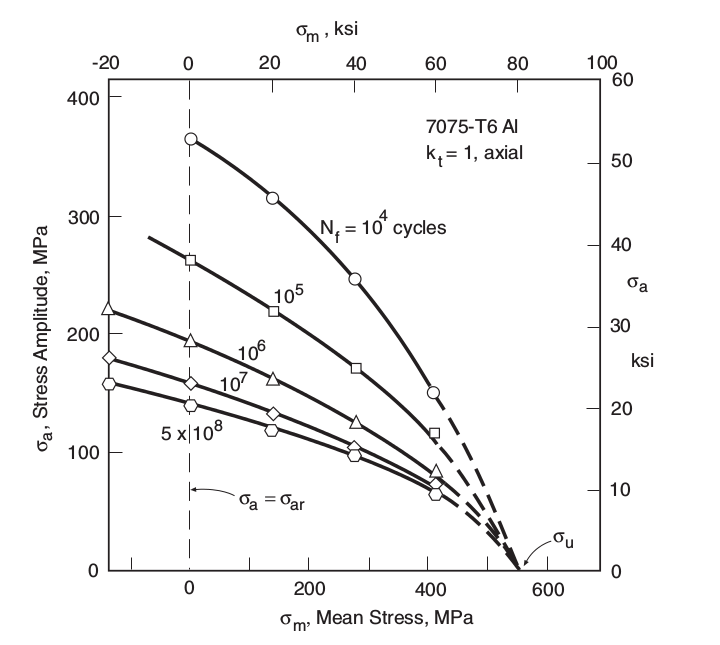
\includegraphics[width=\textwidth]{Imagenes/diag_cfl.png}
\caption{Diagrama de vida constante para aluminio 7075-T6}
\label{fig:diag_cfl}
\end{figure}

\subsubsection{Diseño para esfuerzos uniaxiales fluctuantes}
Cuando elementos están sometidos a esfuerzos repetidos con componentes medios distintos de cero, estos deben tomarse en cuenta para el diseño. Para esto, se utiliza un diagrama de esfuerzo alternante versus esfuerzo normal en el cual se ajustan distintas curvas a los datos obtenidos. Como se muestra en la figura \textcolor{red}{añadir imagen 442 norton pag 324}, existe la línea de Goodman modificada, la parábola de Gerber y la línea de Soderberg. La parábola de Gerber es la que mejor se ajusta a los datos de falla experimental, de acuerdo a la ecuación \ref{eq:gerber}; mientras que la línea de Goodman modificada, ecuación \ref{eq:good_mod}, se ajusta por debajo de la dispersión de datos. Ambas curvas utilizan en el eje $\sigma_a$ el límite de resistencia a la fatiga $S_e$ y el esfuerzo último $S_u$ o $S_{ut}$ en el eje $\sigma_m$. En cambio, la línea de Soderberg, ecuación \ref{eq:soderberg}, une $S_e$ con la resistencia a la fluencia del material $S_y$ y es, por lo tanto, un criterio de falla más conservador que los demás. Sin embargo, la línea punteada que une ambos $S_y$ se debe utilizar en las dos primeras curvas como límite del primer ciclo de esfuerzo para evitar que ceda o falle. \textcolor{red}{Referencia a libro norton}

\begin{centering}
\begin{align}
&\text{Parábola de Gerber:}&	\frac{\sigma_a}{S_e} &+ \frac{\sigma_m^2}{S_u^2} = 1 \label{eq:gerber}\\
&\text{Goodman modificada:}&	\frac{\sigma_a}{S_e} &+ \frac{\sigma_m}{S_u} = 1 \label{eq:good_mod}\\
&\text{Soderberg:}&	\frac{\sigma_a}{S_e} &+ \frac{\sigma_m}{S_y} = 1 \label{eq:soderberg}
\end{align}
\end{centering}



\subsubsection{Diagramas de esfuerzos alternantes normalizados y medios}

La normalización del diagrama mostrado en la figura \ref{fig:diag_cfl} responde a la necesidad de consolidar los datos de mediciones para distintos esfuerzos medios y vida de fatiga dentro una sola curva. Esto da la oportunidad de ajustar la curva a una ecuación que represente todos los datos obtenidos. Así para el caso particular de $S_m=0$, el esfuerzo alternante se designará por $\sigma_{ar}$. Por lo tanto, en el diagrama $CFL$, $\sigma_{ar}$ es el intercepto en $\sigma_m=0$ de la curva para cualquier vida $N_f$. Por consiguiente, el gráfico puede ser normalizado utilizando la relación $\sigma_a/\sigma_{ar}$ en la ordenada y el esfuerzo medio $\sigma_m$ en la abscisa. De esta manera, se cumplirá que $\sigma_a/\sigma_{ar}=1$ cuando $\sigma_m=0$ y, además, cuando el esfuerzo alternante es cercano a cero, el valor del esfuerzo medio debe aproximarse al esfuerzo último del material, $\sigma_u$. El resultado de esto se puede apreciar en la figura \ref{fig:cfl_norm} \textcolor{red}{buscar otra imagen de referencia}.

\begin{figure}[h]
\centering
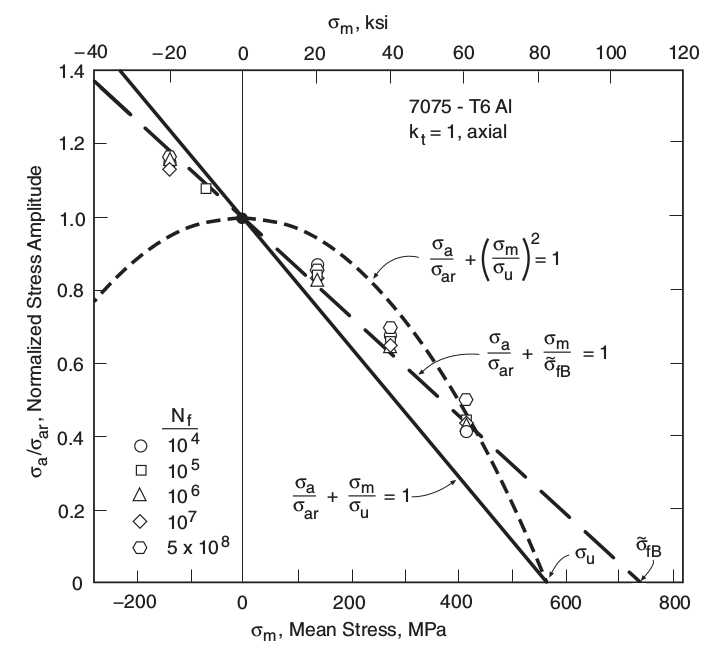
\includegraphics[width=\textwidth]{Imagenes/cfl_norm.png}
\caption{Diagrama CFL normalizado}
\label{fig:cfl_norm}
\end{figure}

Al igual a como se vio en la sección anterior, las curvas que se ajustan a estos valores pueden ser rectas o una parábola. La ecuación modificada de Goodman normalizada sigue siendo una aproximación conservadora, y su versión normalizada es:

\begin{equation} \label{eq:good_norm}
	\frac{\sigma_a}{\sigma_{ar}} + \frac{\sigma_m}{\sigma_u} = 1 
\end{equation}

La parábola de Gerber queda expresada como:

\begin{equation} \label{eq:par_gerber}
	\frac{\sigma_a}{\sigma_{ar}} + \left(\frac{\sigma_m}{\sigma_u}\right)^2 = 1 
\end{equation}

Y una segunda modificación de la ecuación de Goodman, propuesta por J. Morrow, para metales dúctiles, en la cual se reemplaza $\sigma_u$ por el esfuerzo verdadero de fractura corregido $\tilde{\sigma}_{fB}$.

\begin{equation} \label{eq:mod_goodduct}
	\frac{\sigma_a}{\sigma_{ar}} + \frac{\sigma_m}{\tilde{\sigma}_{fB}} = 1 
\end{equation}


\subsection{Medición de la fatiga}
Existen distintas técnicas para cuantificar la respuesta de un material o componente frente a esfuerzos o deformaciones fluctuantes. La primera de ellas, como se habló anteriormente, corresponde a una viga giratoria sometida a flexión en voladizo, diseñada por A. Wöhler. Con respecto a la información existente en la literatura la mayoría de los datos disponibles de resistencia a la fatiga se encuentra en las pruebas de viga giratoria (\textit{rotating bending}, en inglés) en ciclo de flexión invertida, seguido por cargas axiales (\textit{push-pull}, en inglés), flexión en voladizo (\textit{alternating bending}, en inglés) y en menor medida, en las pruebas de fatiga por torsión. \textcolor{red}{citar norton seccion 45}

\subsubsection{Ensayo de fatiga con una viga giratoria en flexión} 
Su uso es el más extendido para determinar la vida a fatiga de un material. La principal ventaja frente a otros sistemas radica en su capacidad de aplicar ciclos de cargas a altas velocidades, es decir, realizar pruebas de fatiga a altas frecuencias. Sin embargo, no es posible aplicar una carga media distinta de cero, por lo tanto, su uso principal se encuentra en la obtención de datos para el rango HCF y de ciclo invertido. Los datos obtenidos son más altos respecto a otros tipos de medición, como se puede ver en la figura REF.


\subsubsection{Ensayo de fatiga axial}
Esta configuración de prueba es más flexible que el resto, siendo posible cualquier combinación de esfuerzo alternante y medio, además de poder realizar ensayos con el modelo de deformación-vida. Su principal diferencia respecto al método de viga giratoria se encuentra en que la sección transversal está sometida a esfuerzos de manera uniforme, provocando que los resultados de resistencia a la fatiga obtenidos sean usualmente menores que las obtenidas por \textit{rotating bending} y \textit{alternating bending}. Se considera que esto se debe a la  probabilidad más alta de hallar una microgrieta en un campo de esfuerzos más grande. Asimismo, la superposición de momentos de flexión sobre las cargas axiales, producto de la dificultad de crear cargas axiales sin excentricidad, son un factor en la disminución en la obtención de valores de resistencia menores. En concreto, la reducción de las resistencias a la fatiga obtenidos pueden variar entre un 10$\%$ y un 30$\%$ o más si hay flexión producto de la excentricidad de las cargas. La figura REF \textcolor{red}{sacar imagen de paper A Esin} muestra las diferencias de los datos obtenidos entre un ensayo de fatiga axial y uno de viga giratorio.

\subsubsection{Ensayo de fatiga de flexión en voladizo}
Esta prueba consiste en someter a una viga en voladizo a oscilaciones en su extremo libre a través de algún mecanismo, pudiendo lograr combinaciones de esfuerzos medios y alternantes. La máquina analizada en esta memoria, utiliza este método para la obtención de los datos de vida de fatiga del material a analizar. Los resultados de este tipo de prueba son inferiores a los obtenidos por \textit{rotating bending} y mayores a los obtenidos por \textit{push-pull}.

\subsection{Correlación entre distintos métodos de medición de la fatiga}
Como se señaló anteriormente y se aprecia en la imagen REF, cada prueba entrega valores distintos aún cuando los niveles de esfuerzo sean iguales. Por esto, existen distintos intentos en la literatura de crear correlaciones entre los datos, evitando los costos asociados a realizar nuevos ensayos experimentales del mismo material o componente. La forma en que se ha abordado esta problemática es la utilización de un factor de corrección ($\phi$) calculado con distintas propuestas.

Algunos de estos modelos son: Manson y Muralidharan, Philipp, Lee y Esin. Cada metodología aborda de distinta forma el cálculo del factor de corrección $\phi$, ahora bien, se abordarán los modelos de Lee y Esin en este trabajo, ya que, de acuerdo a \textcolor{red}{agregar cita de analysis of axial papre}, son los modelos que se ajustan mejor al comportamiento de los datos empíricos entre ensayos de \textit{rotating bending} y de \textit{push-pull}. \textcolor{red}{corregir}

\subsubsection{Modelo de Esin}
El modelo propuesto por Esin en \textit{``A method for correlating different types of fatigue curve"}, relaciona las curvas \textit{push-pull}, \textit{alternating bending} y \textit{rotating bending}. Este depende del esfuerzo alternante, asumiendo que la curva base y la calculada por este método se intersectarán en el punto ($S_e,N_f$), es decir, el factor de correción es $\phi=1$ en esa posición. 

El método se basa en el análisis de la dependencia de la micro-plasticidad en la distribución de esfuerzos en la sección transversal, definiéndose la micro-plasticidad como el flujo plástico de un material sin haber alcanzado su punto de fluencia. Esta ocurre sobre cierto nivel de esfuerzos en el rango elástico, donde ese nivel se llama límite elástico real (\textit{true elastic limit}, en inglés o \textit{tel}) y bajo límite de resistencia a la fatiga, $S_e$. Así, siempre se cumplirá que:
\begin{align*}
	tel \leq S_e \leq S_f
\end{align*}

La micro-plasticidad es un fenómeno altamente localizado que depende de las propiedades probabilísticas micro-estructurales del material como su micro-in-homogeneidad, anisotropía y micro-concentraciones de esfuerzos, los cuales explican la dispersión de datos en los ensayos de fatiga. Así, cuando los esfuerzos alternantes están sobre \textit{tel}, la micro-plasticidad influye en los macro-elementos. Dicho de otra forma, el comportamiento mecánico observado a un nivel macro es el comportamiento integrado de los micro-elementos.

En la figura REF \textcolor{red}{agregar imagen 2 del paper}, se puede apreciar las áreas afectadas por fatiga para cada tipo de ensayo, los cuales, por sí mismo podrían explicar las diferencias en los resultados de cada prueba. Sin embargo, basándose en el criterio de fatiga de la deformación micro-plástica, la falla ocurre cuando la energía acumulada por la histérsis plástica es igual al valor de la energía de ruptura real (área bajo la curva de un diagrama $\sigma$-$\varepsilon$ real).

\begin{equation}\label{eq:esin_n}
	N = \frac{U \cdot T_t}{W} 
\end{equation}

Donde:
\begin{itemize*}
	\item $N$: Número de ciclos a la falla.
	\item $U$: Energía total real bajo la curva del diagrama esfuerzo-deformación.
	\item $W$: Energía total plástica disipada.
	\item $T_t$: Número total de macro-elementos.
\end{itemize*}

De esta forma, el método de correlación utiliza el concepto de esfuerzo alternante equivalente, $S_e'$, utilizado para denotar un esfuerzo hipotético actuando sobre todos los elementos sometidos a fatiga. 
\begin{equation}\label{eq:esfalt_eq}
	S_e' = \frac{\Sigma \sigma_i A_i}{\Sigma A_i}
\end{equation}
Donde $A_i$ es el número o área de los macro-elementos con igual esfuerzo equivalente. A partir de esto, el esfuerzo equivalente para ensayos de \textit{rotating bending} y \textit{alternating bending}, están dados por las ecuaciones \ref{eq:seq_rotben} y \ref{eq:seq_altben}, respectivamente. 

\begin{align}
	S_{e,rt}' &= \frac{2S\cdot \sin^3 \theta}{3C} \label{eq:seq_rotben}\\
	S_{e,ab}' &= \frac{2S}{3} \cdot \left(\frac{1-c^3}{1-c^2}\right) \label{eq:seq_altben}
\end{align}

DEFINIR C y c, escribir factor de fatiga para AB y RB. Describir uso del método. Mostrar imagenes comparativas. FIN.

\subsubsection{Modelo de Lee}
La estimación del límite de fatiga, $S_e$, se calcula a través de distintos factores de modificación según el tipo de carga, calidad superficial, tamaño y confiabilidad de la muestra. El factor de modificación según el tipo de carga $C_L$ varía entre 0,7 y 0,9 para probetas sin muescas. Las recomendaciones para cada valor de $C_L$ se realizaron considerando los efectos del gradiente de esfuerzos y el tipo de esfuerzo involucrado, es decir, cortantes y normales. Estos también varían según el tipo de material, los cuales fueron obtenidos de manera empírica. Así la tabla \ref{tab:lee_factor} muestra los factores de modificación para algunos tipos de carga.


\begin{table}[h]
\centering
\caption{Factores de modificación por tipo de carga, según el modelo de Lee.}
\label{tab:lee_factor}
\begin{tabular}{@{}llc@{}}
\toprule
Tipo de Carga                & $C_L$ & \multicolumn{1}{l}{Observaciones} \\ \midrule
Carga axial pura             & 0,9   & -                                 \\
Carga axial con leve flexión & 0,7   & -                                 \\
Rotating bending             & 1,0   & -                                 \\
Torsional                    & 0,58  & \multicolumn{1}{l}{Para aceros}   \\ \bottomrule
\end{tabular}
\end{table}

Además, es posible apreciar en la imagen REF \textcolor{red}{colocar imagen 416 del texto de Lee} las diferencias que se generan por la aplicación del factor de corrección para los distintos tipos de carga que se buscan. 

AÑADIR IMAGEN COMPARANDO AMBOS SISTEMAS.

\section{Vibraciones}
La vibración es un término que describe el fenómeno de las oscilaciones de un sistema mecánico al rededor de un punto de equilibrio. Es una subdisciplina de la dinámica que estudia el movimiento repetitivo de los cuerpos y las fuerzas asociadas a los mismos.\\
Un sistema vibratorio está compuesto, generalmente, por elementos de masa, elásticos y de amortiguamiento, cada uno de los cuales es un medio para almacenar energía cinética, potencial y de disipar la energía, respectivamente, los cuales se transfieren de manera alternante entre energía potencial y energía cinética.

\subsection{Modelo Matemático}

\subsection{Rigidez}

\subsection{Método de energía}

\subsection{Damping}

\subsection{Vibraciones forzadas}

\subsection{Sistema de dos grados de libertad}

\subsection{Ecuaciones de energía para un sistema con amortiguamiento y forzado}
